\section{Embedded Platform Demonstration}
\label{sec:experiment}

To demonstrate the complete Maverick flow, we targeted Digilent's embedded PYNQ-Z1 board, which contains a Xilinx Zynq xc7z020 SoC, 512 MB of RAM, and a microSD card slot. 
The Zynq device tightly couples a dual-core ARM Cortex-A9 processor to an FPGA fabric.

The PYNQ-Z1 board is designed as a hardware platform for Xilinx's open-source Python Productivity for Zynq (PYNQ) system.
Its ARM CPU runs Ubuntu Linux, the open-source Jupyter notebook infrastructure, and a web server.
The PYNQ system can be accessed from any computing platform and operating system via a web interface.

We believe PYNQ is an ideal candidate for a stand-alone system using Maverick.
In our demonstration, the Maverick RM CAD flow runs on the Zynq's ARM processing system (PS) to compile HDL designs to partial bitstreams for the Zynq's programmable logic (PL). 
The PYNQ Python interface running on the ARM processor then programs those bitstreams onto the PL.

\subsection{PYNQ-Z1 Setup}
\label{sec:pynqSetup}

\begin{figure}
	\centering
	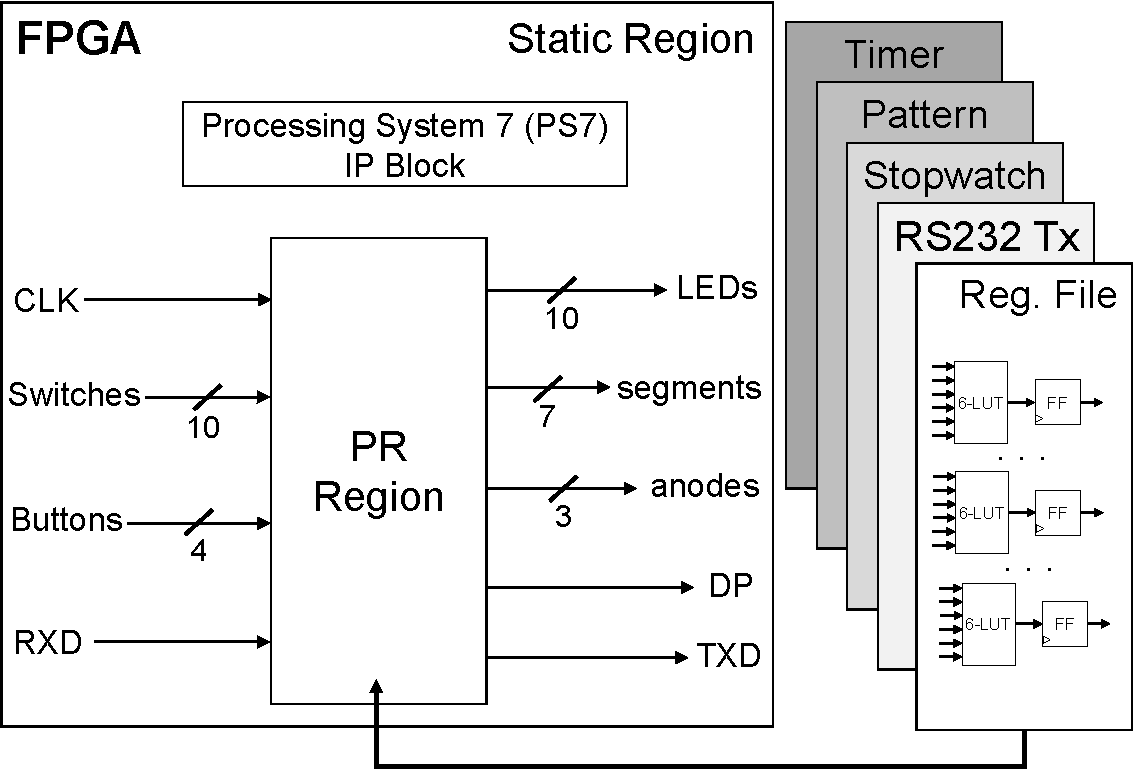
\includegraphics[width=.82\columnwidth,keepaspectratio]{figures/pynq_rp}
	\caption{The Static Design Used in the PYNQ-Z1 Demonstration}
	\label{fig:pynq_rp}
\end{figure}

To prepare our demonstration, we first created a static design, as described in Section~\ref{sec:static_system}. 
As shown in \figurename~\ref{fig:pynq_rp}, the static region included the Processing System 7 (PS7) IP core, which acts as a logical connection between the Zynq's PS and PL \cite{Xilinx:2017}. 
In addition, the static region contained clocking and various I/O interfaces (for buttons, a seven segment display, RS232 signals, etc.) which the PR region connects to.
The PR region was made up of 8 columns by 50 rows of configurable logic block (CLB) and interconnect tiles, following the vertical and horizontal alignment rules required by the Xilinx 7-Series architecture \cite{Xilinx:2018d}. 

\begin{figure*}[htb]
	\centering
	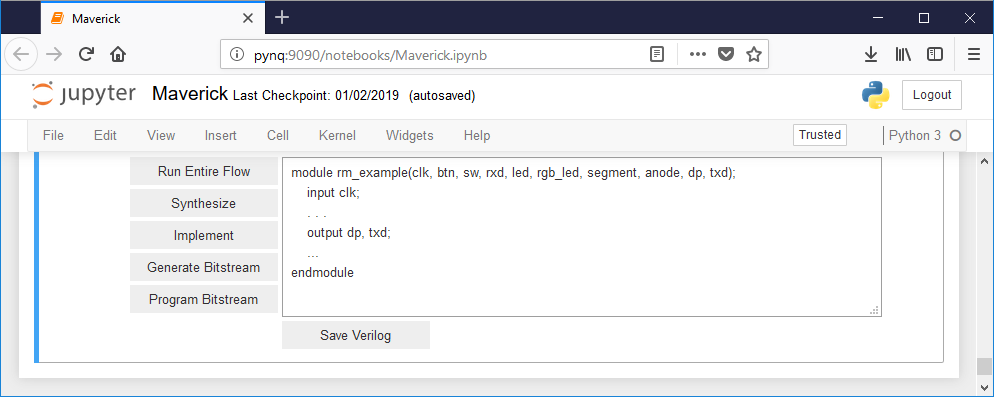
\includegraphics[width=.85\textwidth,keepaspectratio]{figures/notebook.png}
	\caption{Jupyter Notebook for the Maverick Flow}
	\label{fig:notebook}
\end{figure*}

We next created a Jupyter notebook, as shown in \figurename~\ref{fig:notebook}.
This notebook makes it possible to create a new design, execute each step of the Maverick design flow on that design, and then program the resulting bitstream onto the FPGA fabric, all within a web interface. 
Verilog designs already saved on the PYNQ-Z1's microSD card can also be used in this notebook.
Alternatively, the Maverick tools could be run using the Ubuntu command line instead. 

We then installed all the required software onto the PYNQ SD card.
This included Yosys, our modified version of RapidSmith2, Project X-Ray, Python 3.5.1, and Oracle's JRE 1.8.
Yosys required 22 MB of storage, RapidSmith2 took 6 MB, and the Project X-Ray tools required 2 MB.
Additionally, we copied the static design metadata (the partial device model, reserved resource list, bitstream database, and initial partial bitstream) to the PYNQ system.  
Furthermore, we replaced the PYNQ-Z1's default Zynq boot image so the FPGA is immediately programmed with our initial full bitstream on boot up.
Once the PYNQ-Z1 finishes its complete boot process, a user can immediately code, implement, and program new RM designs onto the PR region of the FPGA.

\subsection{Benchmark Design Results}
\label{sec:results}

To test the Maverick flow, we created a set of five benchmark Verilog designs that might be designed as part of an introductory digital systems course, including: (1) an 8x6-bit register file, (2) an RS232 transmitter, (3) a 7 segment display stopwatch, (4) an input pattern game, and (5) a response timer game.
Furthermore, these designs could be used in an educational setting on PYNQ in which a Jupyter notebook could mix instructional materials, sample designs, HDL code, and CAD tools into an interactive learning environment.
The designs all use physical I/O such as buttons, switches, and LEDs to enable students to interact with and verify the proper operation of the designs.
Not all device features are supported by Maverick and so these designs only require slices to implement.

\begin{figure}
	\centering
	\includegraphics[width=.52\columnwidth,keepaspectratio]{figures/board}
	\caption{The PYNQ-Z1 Board Configured with a Stopwatch Partial Bitstream Generated by Maverick}
	\label{fig:board}
\end{figure}

We used the Maverick Jupyter notebook to run each of our benchmark designs through the full Maverick flow, all on the Zynq device's ARM CPU.
Following the bitstream generation of each design, an API added to the PYNQ system \cite{Goeders:2018} was used to partially reconfigure each design onto the Zynq's PL. 
Then, we functionally tested each design and verified their correct operation in hardware.
\figurename~\ref{fig:board} shows the PYNQ-Z1 board after it was partially reconfigured with a partial bitstream for the stopwatch design, which was generated by the Maverick flow. 

Additionally, we measured the run time for each benchmark design as it ran through each major step of the Maverick flow.
\figurename~\ref{fig:runtime} presents the run time results for each step running on the PYNQ-Z1's ARM CPU, which runs at 650 MHz. 
We also measured the run times for each step of the Maverick flow on a desktop computer with an Intel i7 860 CPU, which runs at 2.80 GHz.
For our benchmark designs, the Maverick flow executed from 6x to 11x slower on the PYNQ-Z1's ARM CPU.
Given the difference in CPU speeds and architectures, we found this to be unsurprising. 

\begin{figure}
	\centering
	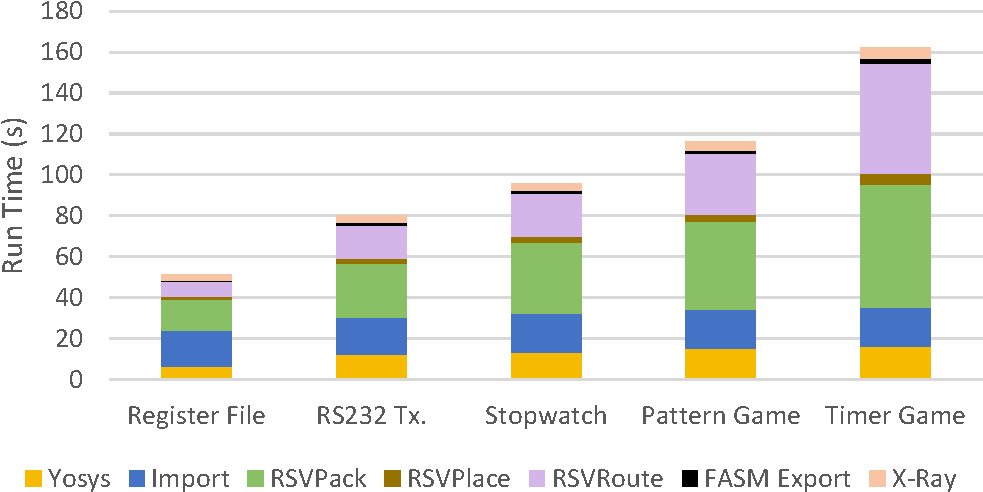
\includegraphics[width=\columnwidth]{figures/runtime}
	\caption{Run Times on the PYNQ-Z1}
	\label{fig:runtime}
\end{figure}

Furthermore, we measured the peak memory usage for each major step of the Maverick flow as it executed on the PYNQ-Z1's ARM CPU. 
The iPython kernel and web server require roughly 120 MB of RAM, leaving 392 MB for the Maverick flow.
For the largest design we tested, Maverick required a maximum of 230 MB of RAM. 
Specifically, Yosys required 24 MB, the RapidSmith2-based programs 230 MB, and the Project X-Ray tools 14 MB of RAM.

To measure the resource utilization for the benchmarks compiled by the Maverick flow, we used the Vivado Design Interface (VDI) \cite{Townsend:2017b} (which was modified to support RM designs) to import each completed RM design into Vivado; we then measured the FPGA resource utilization for each.
Additionally, we compiled each RM design using only Vivado's PR flow and measured the resulting resource utilization for each design.
Table~\ref{tab:tab1} compares the resulting FPGA resource utilization from the Maverick flow and from Vivado's PR flow.
Note that the number of used LUTs in this table includes the LUTs in the netlist, LUTs used as route-throughs, and LUTs used as VCC or GND sources.

While Vivado was clearly able to produce better results, we still find these results to be promising and acceptable for use in a small embedded system.
The run times to fully compile the designs on the PYNQ-Z1's ARM processor were all on the order of a few minutes at most.
Additionally, the amount of RAM available for use by Maverick, roughly 392 MB, was almost double the RAM required for the designs we tested.
These results demonstrate the feasibility of running a stand-alone FPGA CAD tool flow on a resource-constrained platform such as the PYNQ-Z1, on which RMs can both be compiled and then programmed onto its own programmable fabric.

\begin{table}[t]
	\caption{Benchmark Design FPGA Resource Utilization}
	\label{tab:tab1}
	\begin{center}
		\begin{tabular}{|l|cc|cc|cc|}
			\toprule
			\multirow{2}{*}{}&\multicolumn{2}{c|}{Slices}&\multicolumn{2}{c|}{LUTs}&\multicolumn{2}{c|}{Flip-Flops}\\
			&Mav.&Viv.&Mav.&Viv.&Mav.&Viv.\\
			\midrule
			Register File & 28 & 21 &47 & 26 & 9 & 9\\
			RS232 Tx. & 53 & 42 & 174 & 114 & 55 & 48\\
			Stopwatch & 57 & 46 & 232 & 136 & 67 & 65\\
			Pattern Game & 79 & 58 & 319 & 187 & 117 & 109\\
			Timer Game & 105 & 73 & 589 & 233 & 128 & 127\\
			\midrule
			PR Region & \multicolumn{2}{c|}{400} & \multicolumn{2}{c|}{3200} & \multicolumn{2}{c|}{3200}\\
			xc7z020clg400-1 & \multicolumn{2}{c|}{13300} & \multicolumn{2}{c|}{106400} & \multicolumn{2}{c|}{106400}\\
			\bottomrule
		\end{tabular}
	\end{center}
\end{table}
